La nostra architettura utilizza il framework Express ed il servizio di database fornito da Firebase (Firestore). Il funzionamento della nostra applicazione si basa su un'architettura three-tier$^{*}$ costituita da:
\begin{itemize}
	\item Client: tramite il Web Browser$^*$, effettua le richieste HTTP all'applicazione;
	\item Server: avvia il framework Express che ``smista" le richieste tra i Presenter di Colletta in ascolto;
	\item Firebase: contiene e mantiene il database in cloud.
\end{itemize}

Colletta è suddivisa in tre parti: model (che gestisce le operazioni sul database), presenter (che gestisce la logica dell'applicazione) e view (che gestisce la visualizzazione delle pagine web). Il sistema permette:
\begin{itemize}
	\item lo svolgimento di esercizi di analisi grammaticale (e ottenimento di una valutazione automatica) e la scrittura dei dati, come ad esempio la soluzione, su un database Firestore messo a disposizione da Firebase;
	\item la visualizzazione e l'utilizzo di un software di apprendimento automatico per il riconoscimento delle classi grammaticali delle parole di una frase.
\end{itemize}

\begin{figure}[h]
	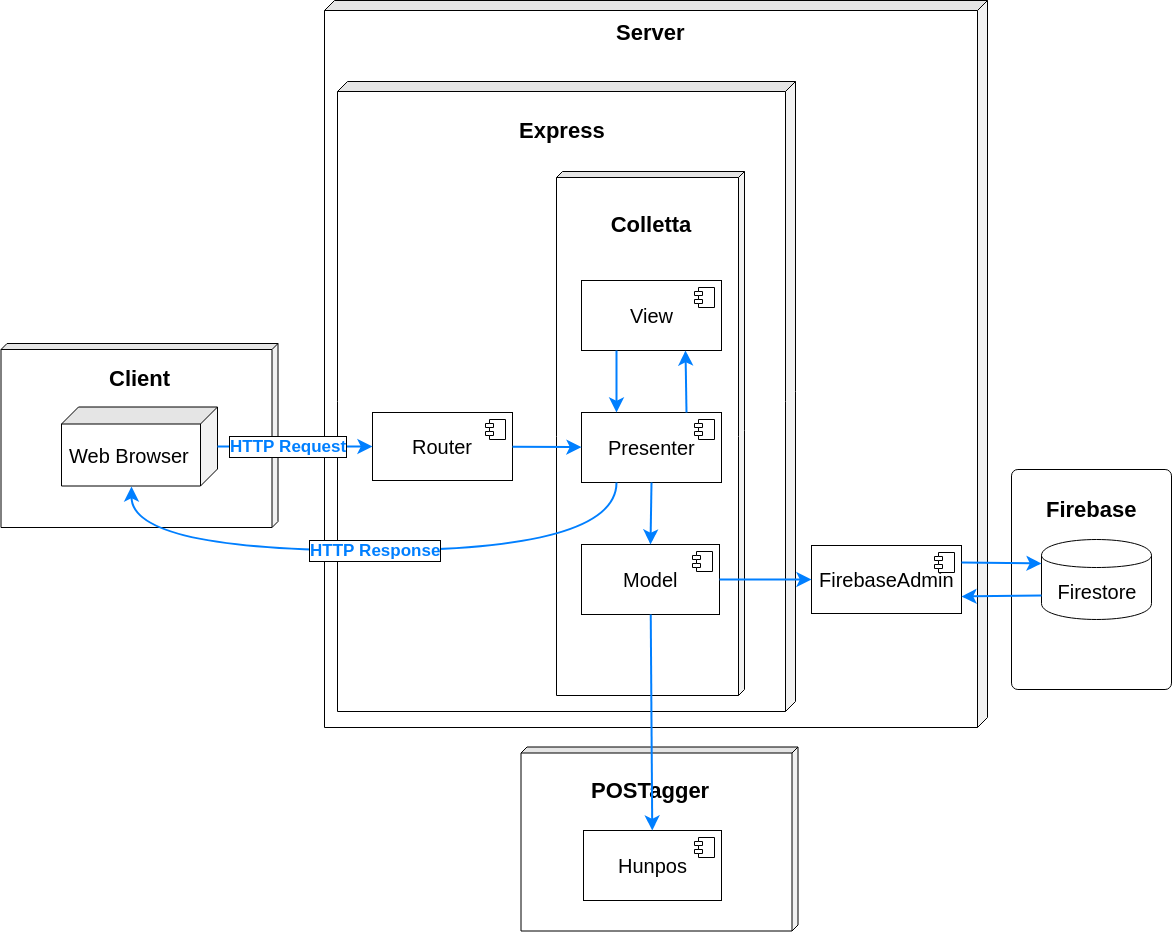
\includegraphics[scale=0.4]{images/architettura.png}
	\caption{Schema generale dell'applicazione}
\end{figure}

\paragraph*{Routing\\}
\noindent Il routing è realizzato dal framework Express e le richieste HTTP vengono smistate tra i vari presenter dell'applicazione, secondo il pattern Model-View-Presenter, ovvero:
\begin{enumerate}
	\item le routes inviano le richieste dell'utente che vengono realizzate da uno specifico presenter;
	\item i presenters operano sul modello, ottengono i dati necessari alla visualizzazione delle pagine e le costruiscono;
	\item le views sono passive e definiscono come sono costituite le varie pagine che verranno visualizzate dall'utente.
\end{enumerate}

\subparagraph*{Routes di visualizzazione}
\begin{itemize}
	\item \texttt{/home}: visualizza la vista principale dell'applicazione, con una barra di input di testo per lo svolgimento di un esercizio;
	\item \texttt{/profile}: visualizza il profilo dell'utente autenticato;
	\item \texttt{/exercise}: visualizza un form per lo svolgimento di un esercizio;
	\item \texttt{/exercise/insert}: visualizza un form per l'inserimento di un esercizio;
	\item \texttt{/registration}: visualizza un form per la registrazione alla piattaforma;
	\item \texttt{/class}:
	\item \texttt{/developer}:
	\item \texttt{/classes}:
	\item \texttt{/exercises}:
	\item \texttt{/exercise/search}:
	\item \texttt{/student/insert}:
	\item \texttt{/class/exercise/search}:
\end{itemize}

\subparagraph*{Routes di utilità}
\begin{itemize}
	\item \texttt{/checklogin}: permette di controllare l'identità di un utente che ha richiesto l'autenticazione;
	\item \texttt{/saveuser}: permette la scrittura delle credenziali di un utente nel database;
	\item \texttt{exercise/save}: permette la scrittura dei dati di un esercizio nel database;
	\item \texttt{/deletestudent}:
	\item \texttt{/deleteexercise}:
	\item \texttt{/addstudent}:
	\item \texttt{/addexercise}:
	\item \texttt{/checkdeveloper}:
	\item \texttt{/download}: ??? CHIEDERE A PERRY O GIAN
	\item \texttt{/download\%model}: ??? CHIEDERE A PERRY O GIAN
	\item \texttt{/exercise/update}:
	\item \texttt{/insertclass}:
	\item \texttt{/deleteclass}:
	\item \texttt{/update}:
	\item \texttt{/logout}:
	\item \texttt{/searchexercise}:
	\item \texttt{/searchstudent}:
	
	
\end{itemize}
\newpage

\subsection{Organizzazione della base informativa}
La base informativa è incentrata sui dati più importanti per la nostra applicazione, ovvero esercizi, classi e utenti. Ogni esercizio salvato nel database ha, inoltre, una o più soluzioni.

\begin{itemize}
	\item \texttt{Exercise}: ogni esercizio viene identificato da un codice e possiede una frase (univoca all'interno del database);
	\item \texttt{Class}: ogni classe viene identificato da un codice, possiede un nome (univoco) e dei riferimenti agli studenti, all'insegnante e agli esercizi ad esso assegnati;
	\item \texttt{User}: ogni utente viene identificata da un codice, possiede dei dati personali (come nome, cognome, città, scuola) e le credenziali di accesso; inoltre, se l'utente non è un insegnante il campo \texttt{teacher} contiene \texttt{-1}.
\end{itemize}

\begin{figure}[ht]
	\centering
	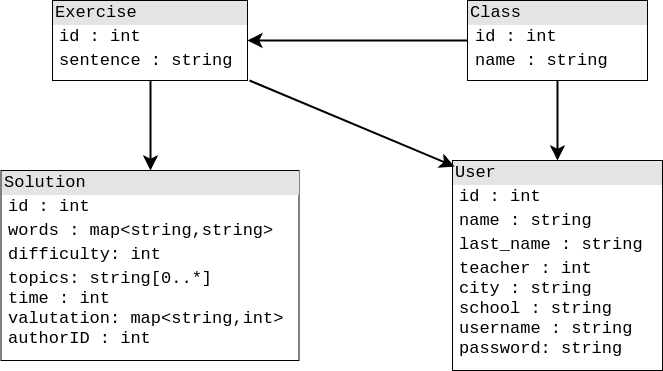
\includegraphics[scale=0.65]{images/database.png}
	\caption{Schema della base informativa}
\end{figure}
\newpage

\subsection{Organizzazione dei packages}
Più in dettaglio, abbiamo suddiviso ulteriormente il model in:
\begin{itemize}
	\item POSManager: parte dell'applicazione che si occupa dell'uso del software di apprendimento automatico;
	\item Data: l'insieme delle classi di business che permettono di svolgere le operazione di calcolo sui dati estratti dal database;
	\item Firebase: insieme di classi usate per l'utilizzo del database fornito da Firebase;
	\item Database: insieme di classi che utilizzano quelle definite dal pacchetto Firebase e che disaccoppiano l'applicazione dall'implementazione del database;
	\item Client: il cui scopo è esporre le funzionalità del model.
\end{itemize}
\begin{figure}[h]
	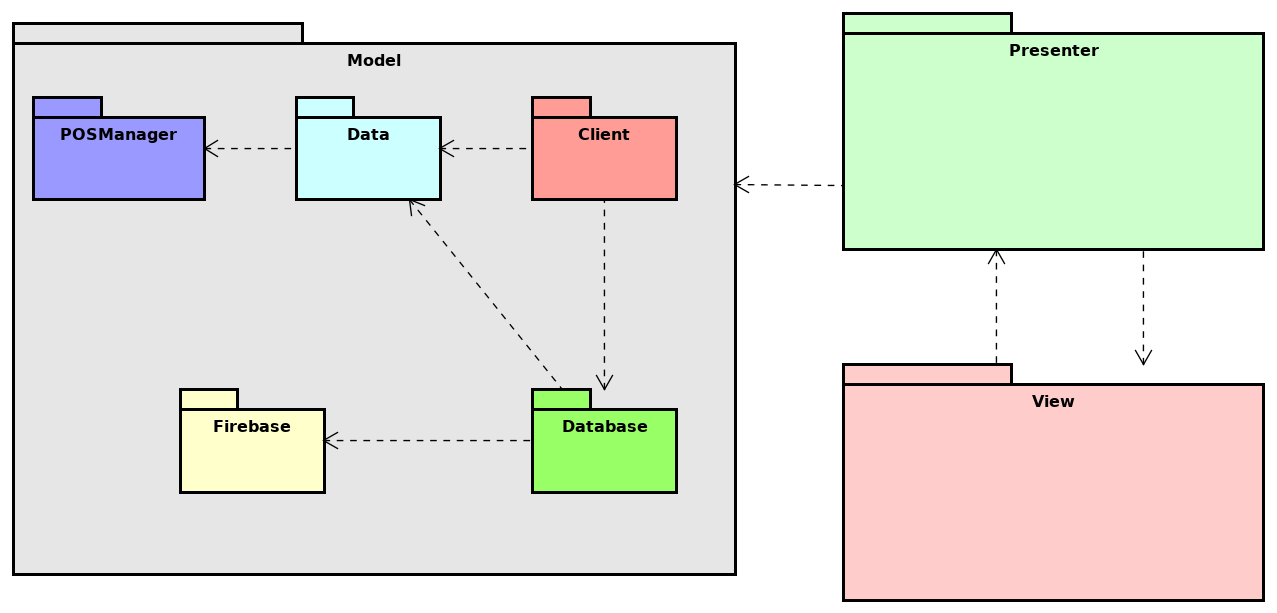
\includegraphics[scale=0.5]{images/package.png}
	\caption{Diagramma dei package}
\end{figure}
\newpage

\subsection{View}
Le viste sono organizzate seguendo una classe base che definisce la struttura di base di una qualsiasi pagina HTML dell'applicazione.
\begin{itemize}
	\item \texttt{DeveloperView}: la vista dedicata allo sviluppatore che necessita di consultare i dati contenuti nella piattaforma; 
	\item \texttt{ProfileView}: la vista dedicata alla visualizzazione del profilo personale e alle relative informazioni (ad esempio, la media degli esercizi per lo studente e il numero di esercizi assegnati per l'insegnante);
	\item \texttt{SearchView}: la vista dedicata alla visualizzazione delle pagine di ricerca della piattaforma;
	\item \texttt{ExerciseView}: la vista dedicata allo svolgimento e all'inserimento degli esercizi nella piattaforma.
\end{itemize}

\begin{figure}[h]
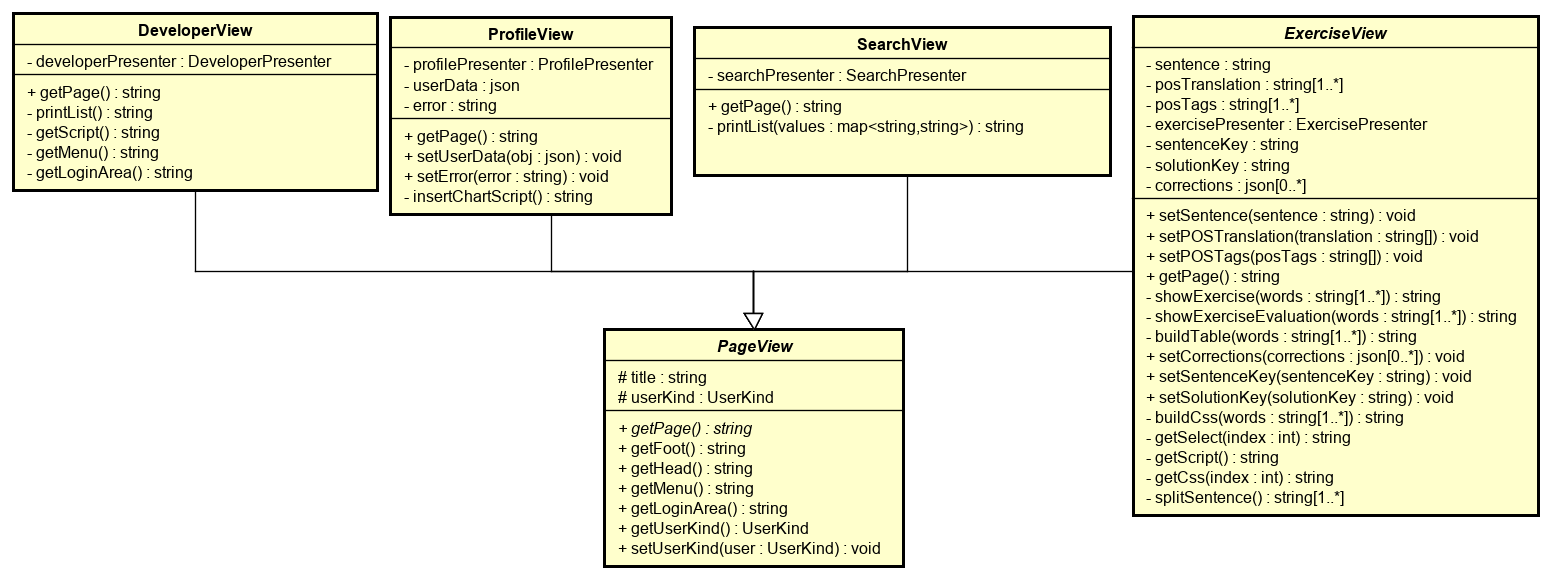
\includegraphics[scale=0.41]{images/View.png}
\caption{Diagramma delle classi di View}
\end{figure}

\newpage

\subsection{Presenter}
I presenter sono organizzati specularmente alle viste ed espongono le funzionalità necessarie per le pagine che gestiscono e definiscono la logica di controllo prelevando le informazioni dal modello. La classe base espone un metodo \texttt{update} che, usando Express, provoca l'aggiornamento della vista. Per offrire le funzionalità alle viste, i presenter hanno un riferimento alla vista e uno al modello dei dati.
\begin{itemize}
	\item \texttt{DeveloperPresenter}: il presenter dedicato alle funzionalità dello sviluppatore che necessita di consultare i dati ed il loro storico;
	\item \texttt{ProfilePresenter}: il presenter che si occupa di recuperare le informazioni legate a un singolo utente (ad esempio, la media degli esercizi per lo studente o il numero di esercizi assegnati per l'insegnante)
	\item \texttt{SearchPresenter}: il presenter dedicato alle funzionalità di ricerca nella piattaforma, come quella degli utenti e degli esercizi;
	\item \texttt{ExercisePresenter}: il presenter dedicato allo svolgimento e all'inserimento di un esercizio nella piattaforma.
\end{itemize}

\begin{figure}[h]
	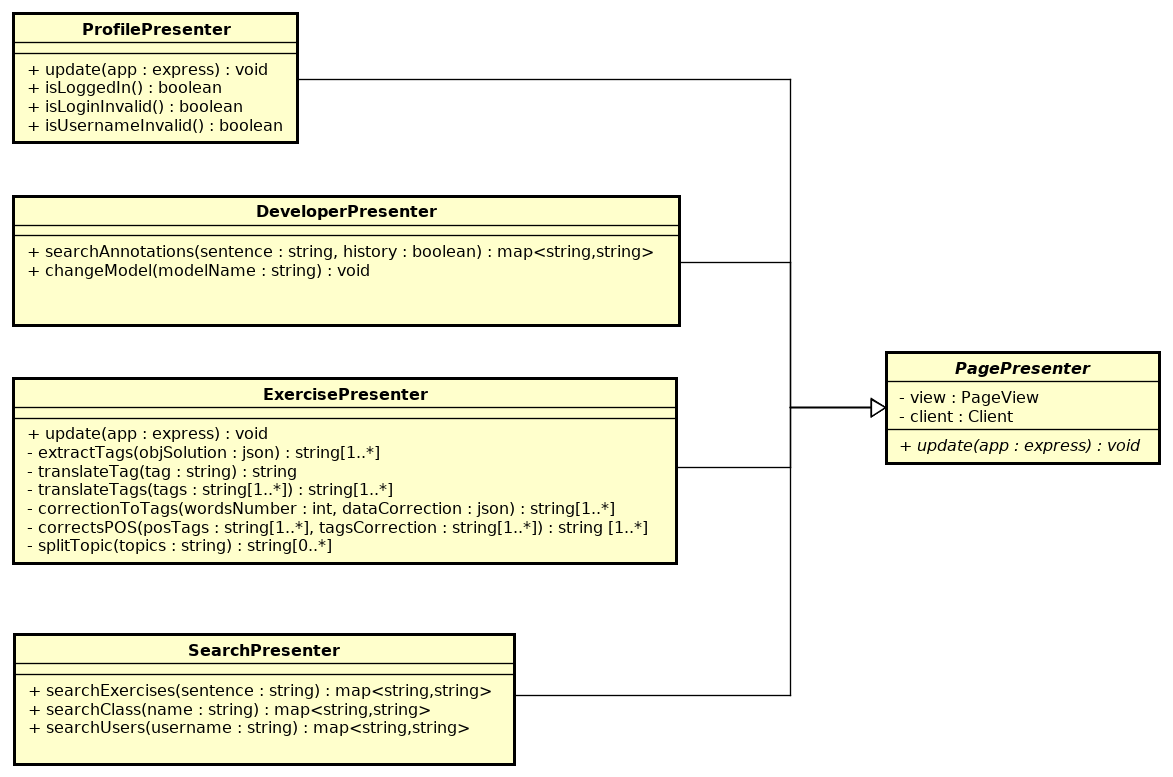
\includegraphics[scale=0.53]{images/Presenter.png}
	\caption{Diagramma delle classi del package Presenter}
\end{figure}

\newpage
\subsection{Model}
\subsubsection{Data}
\begin{figure}[ht]
	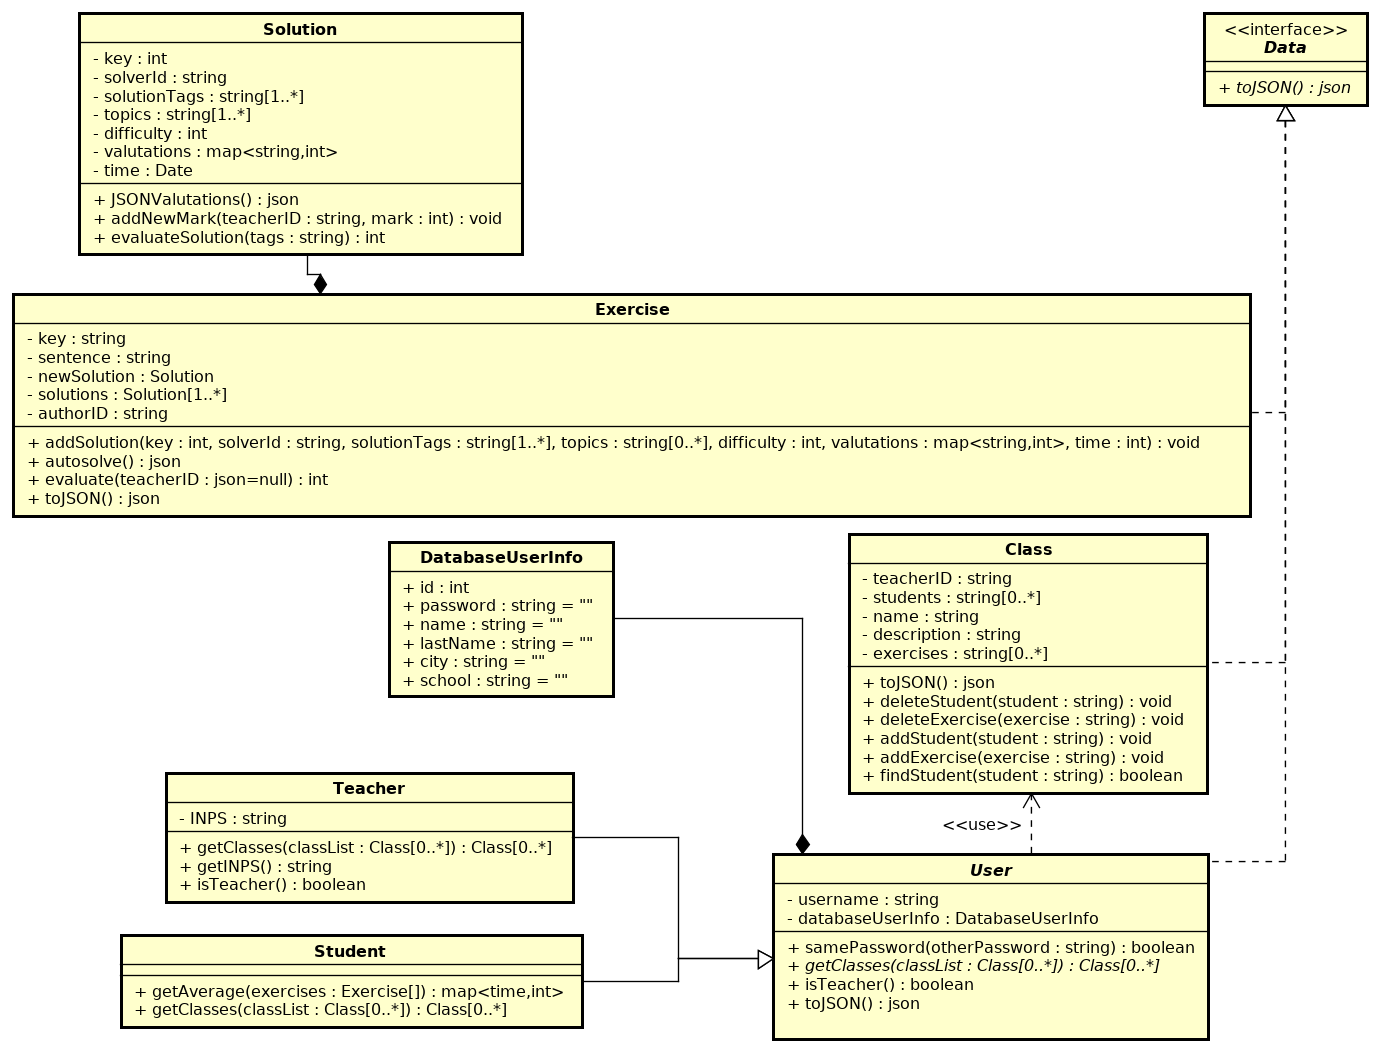
\includegraphics[scale=0.45]{images/Data.png}
	\caption{Diagramma delle classi del package Data}
\end{figure}

In Data si trovano tutte le classi di business dell'applicazione che permettono di calcolare valutazioni di esercizi, medie degli utenti e la risoluzione degli esercizi. Le classi rispecchiano la rappresentazione della base informativa.

\begin{itemize}
	\item \texttt{Data}: interfaccia che identifica tutti i dati rappresentati nel database;
	\item \texttt{Exercise}: modellazione di un esercizio presente nel database che espone le funzionalità necessarie allo svolgimento e alla valutazione di un esercizio da parte di un particolare insegnante;
	\item	\texttt{Solution}: modellazione di una soluzione di un esercizio che permette la valutazione della soluzione;
	\item \texttt{Class}: modellazione delle classi contenute nella piattaforma che mette in relazione studenti e insegnanti;
	\item \texttt{User}: modellazione di un utente qualsiasi registrato nella piattaforma che permette il calcolo delle informazioni correlate a tali utenti:
	\begin{itemize}
		\item \texttt{Teacher}: modellazione di un insegnante che permette il calcolo delle classi di cui esso è insegnante;
		\item \texttt{Student}: modellazione di uno studente che permette il calcolo dell'andamento della media delle valutazioni e delle classi a cui appartiene.
	\end{itemize}
\end{itemize}


\subsubsection{POSManager}
POSManager fornisce il modo di svolgere esercizi tramite il software di POS-tagging. Il pacchetto fornisce un'interfaccia che ogni software di questo tipo deve soddisfare, ovvero le operazioni di training e tagging e la capacità di restituire il risultato di quest'ultima operazione. In particolare, HunposManager è dotato di ulteriori funzioni che permettono la costruzione della soluzione. 

\begin{figure}[ht]
	\centering
	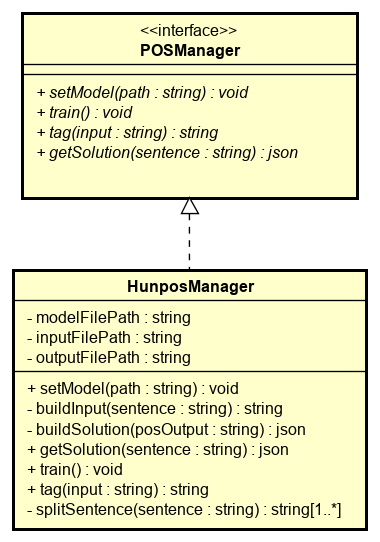
\includegraphics[scale=0.5]{images/POSManager.png}
	\caption{Diagramma delle classi del package POSManager}
\end{figure}
\newpage

\subsubsection{Database}
Database gestisce l'utilizzo del database tramite le classi DatabaseManager e derivate. La suddivisione rispecchia la rappresentazione dei dati all'interno della base di dati. In particolare:
\begin{itemize}
	\item \texttt{DatabaseExerciseManager}: permette le operazioni CRUD$^{*}$ e di ricerca degli esercizi;
	\item \texttt{DatabaseClassManager}: permette le operazioni CRUD e di ricerca delle classi;
	\item \texttt{DatabaseUserManager}: permette le operazioni CRUD e di ricerca degli User.
\end{itemize}
Questa gerarchia di classi agevola, in caso di ristrutturazione dell'applicazione, la sostituzione della base di dati dell'applicazione, semplicemente cambiando il riferimento al database. In questo caso, sarà necessario modificare il riferimento della classe al database. Tale modifica sarà però circoscritta a questa gerarchia di classi senza alcuna necessità di modificare le altre classi dell'applicazione.
\begin{figure}[h]
	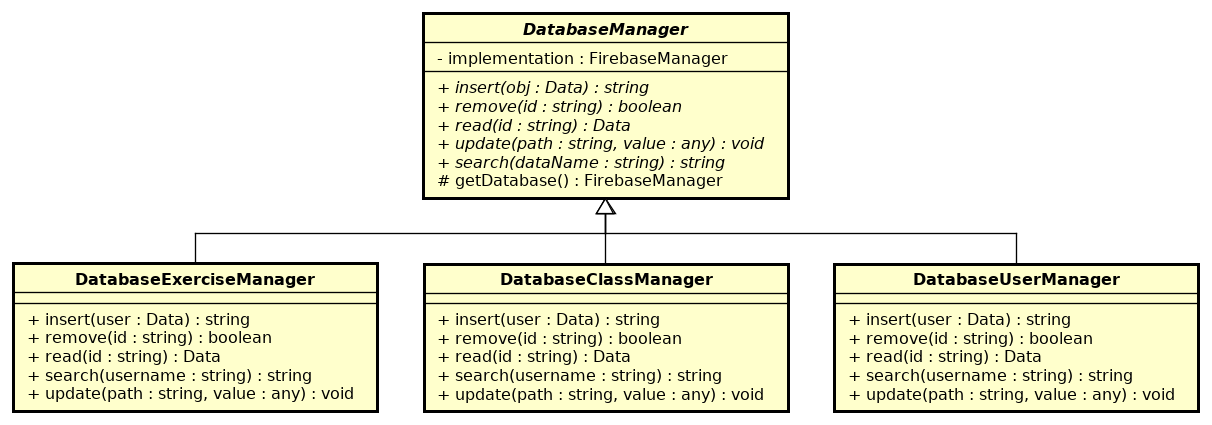
\includegraphics[scale=0.5]{images/DatabaseManager.png}
	\caption{Diagramma delle classi del package Database}
\end{figure}

\newpage
\subsubsection{Firebase}
Firebase rappresenta l'implementazione del database dell'applicazione e permette l'uso del database Firestore fornito da Firebase. In particolare:
\begin{itemize}
	\item \texttt{FirebaseExerciseManager}: permette le operazioni CRUD e di ricerca degli esercizi su Firestore;
	\item \texttt{FirebaseClassManager}: permette le operazioni CRUD e di ricerca delle classi su Firestore;
	\item \texttt{FirebaseUserManager}: permette le operazioni CRUD e di ricerca degli User su Firestore.
\end{itemize}

\begin{figure}[h]
	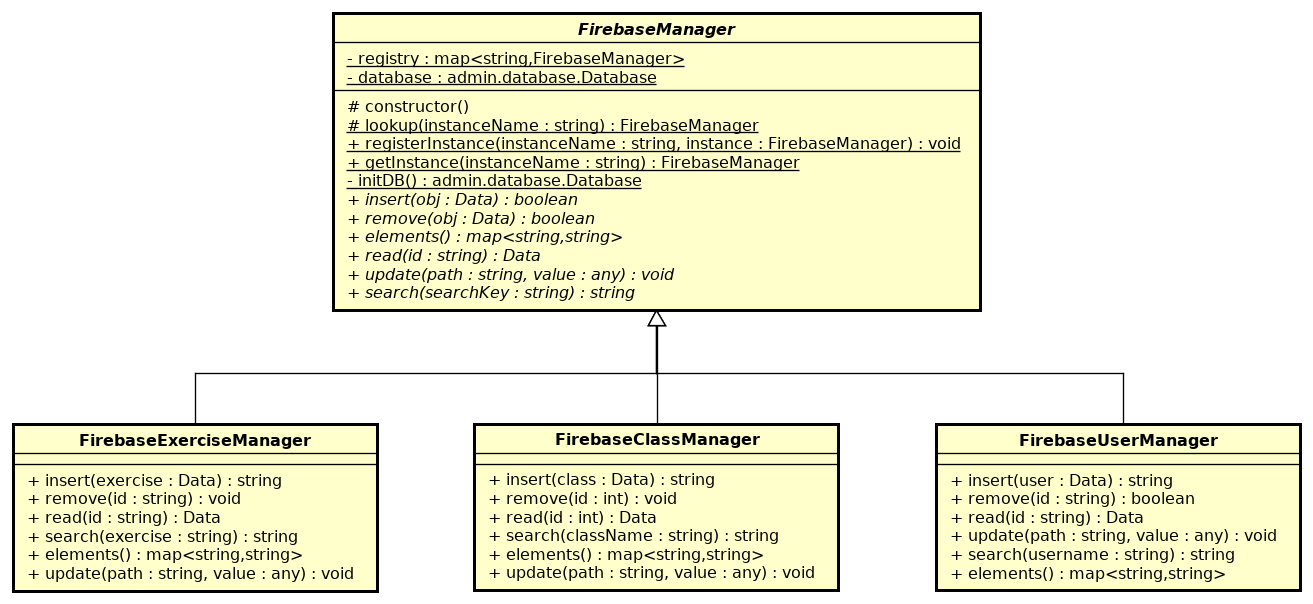
\includegraphics[scale=0.5]{images/FirebaseManager.png}
	\caption{Diagramma delle classi del package Firebase}
\end{figure}

\newpage
\subsubsection{Client}
Client è composto da diverse classi che espongono le varie funzionalità sul modello. In particolare, la classe \texttt{Client} è una composizione di funzionalità fornite da:
\begin{itemize}
	\item \texttt{ExerciseClient}: fornisce le funzionalità di inserimento, risoluzione e ricerca degli esercizi;
	\item \texttt{ClassClient}: fornisce le funzionalità di inserimento e recupero delle informazioni delle classi e l'assegnazione degli esercizi;
	\item \texttt{UserClient}: fornisce le funzionalità di inserimento e verifica dell'identità degli utenti.
\end{itemize}

\begin{figure}[ht]
	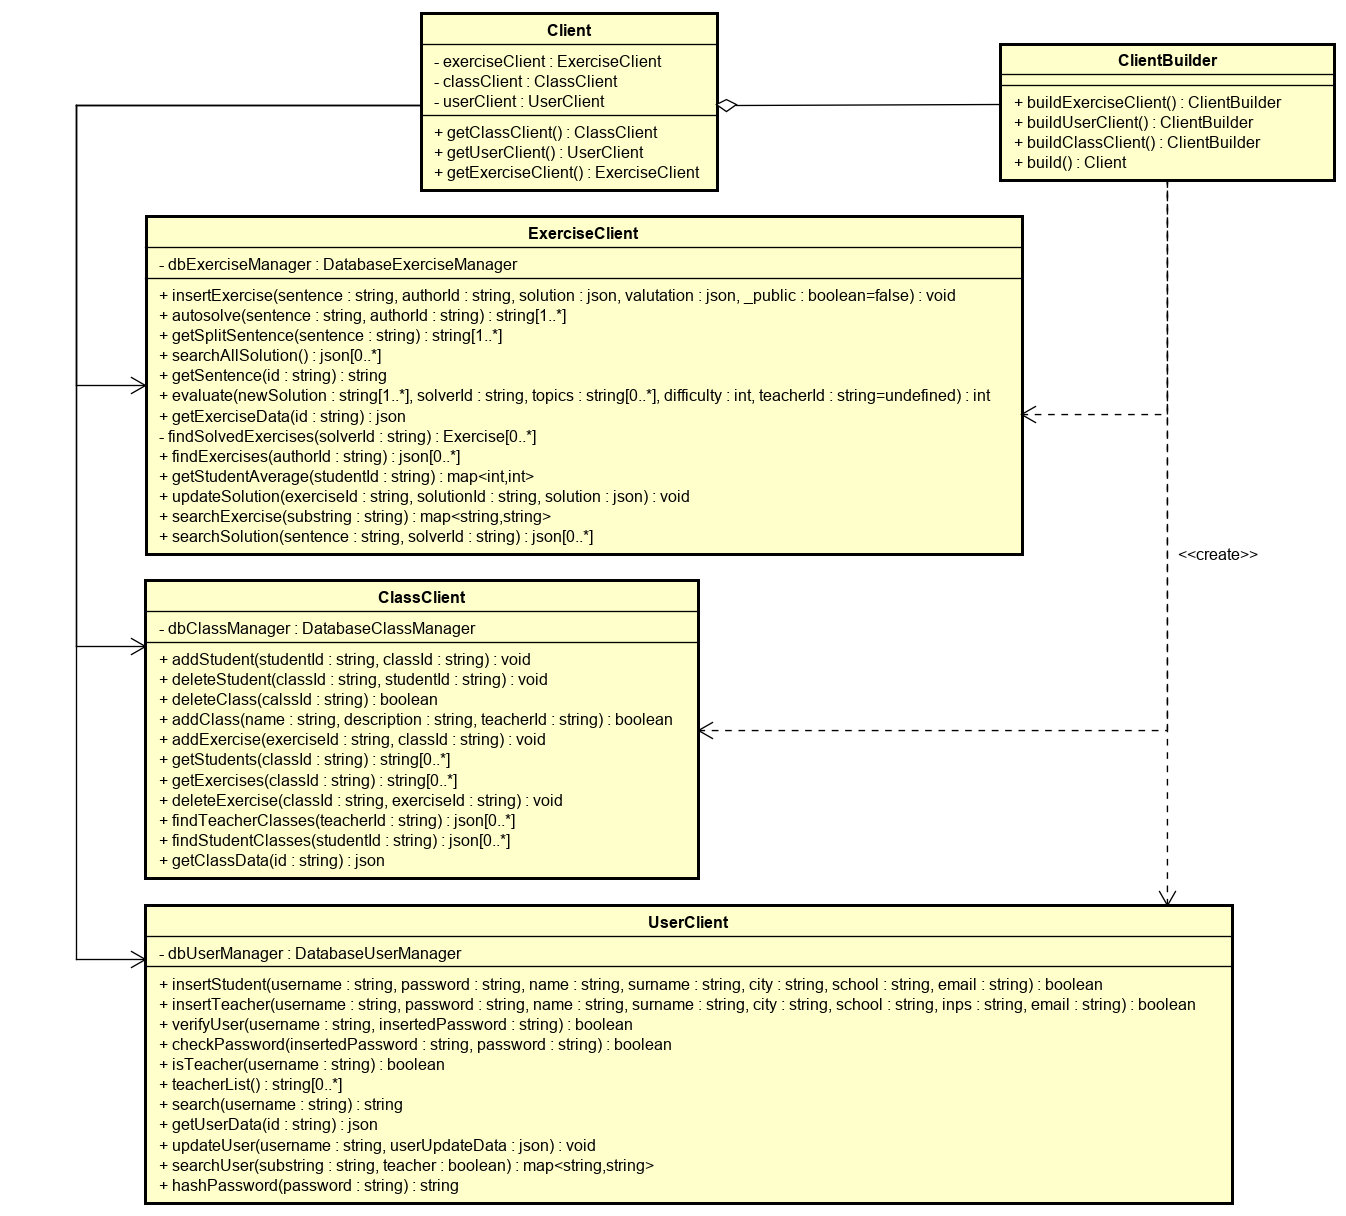
\includegraphics[scale=0.5]{images/Client.png}
	\caption{Diagramma delle classi del package Client}
\end{figure}


\newpage